\chapter{Las últimas pinceladas}
\label{sec:texto}

\lettrine[lines=2]{A}{l día siguiente} Cecilia no entró sola a la
oficina de Antonia: la acompañaba una fragante docena de
medialunas. Su amiga, por primera vez en mucho tiempo, despejó de
papeles el escritorio: tal compañía merecía un lugar especial.

El Sol asomaba sus rayos por la amplia ventana que daba a los
jardines, sumando su calidez al ambiente festivo que producían las
risas contagiosas de ambas amigas. Reían con la facilidad que permite
la amistad, sin que lo exija un chiste u observación demasiado
ocurrente. Simplemente se sentían dichosas.

Cuando la docena se transformó en seis, Antonia se limpió un poco los
dedos en uno de los papeles periféricos del escritorio y se dispuso a
proponer los últimos retoques al reloj de Sol di\-gi\-tal:

---Quedamos en ofrecer al usuario la posibilidad de crear dos tipos de
relojes: uno que sólo muestre unas cuantas horas puntuales escogidas
por él, y otro que presente todas las que abarcan desde las 9:00 a las
15:10 ---recordó.

Cecilia, recostada contra el respaldo de la silla, saboreó ese
recuerdo casi con la misma fruición con la que terminaba su tercera
medialuna.

---¿No sería más lindo ofrecerle un solo módulo, y que éste se
encargue de hacer un reloj u otro? ---preguntó Antonia con tono
evidentemente retórico.

---¿Vos decís que escribamos un módulo que lea la mente?  ---Cecilia
seguía de excelente humor, y sólo parecía querer tener otra excusa
para reír.

---No estaría mal ---respondió Antonia con una son\-ri\-sa---.  Pero
yo estaba pensando en algo más modesto: crear un módulo
\lstinline!reloj_de_sol! que examine los parámetros que recibe: en el
caso de que no reciba ninguno, que cree un
\lstinline!reloj_de_sol_continuo!; y si recibe un vector, que produzca
un \lstinline!reloj_de_sol_discreto!.

---Suena bien ---asintió Cecilia.

\section{Parámetros indefinidos}

Antonia no había esperado la aprobación de su amiga para empezar a
escribir.

\begin{lstlisting}
/* Crea un reloj de Sol en funcion
   del valor de 'vector_horas'.
   Ver comentarios en los modulos
   'reloj_de_sol_continuo' y
   'reloj_de_sol_discreto'.
*/
module reloj_de_sol(vector_horas){
  if(vector_horas==undef)
    reloj_de_sol_continuo();
  else
    reloj_de_sol_discreto(vector_horas);
}
\end{lstlisting}

---Creo que el texto se explica solo ---el optimismo de Antonia seguía
intacto---. En la línea 8 se indaga si el usuario invocó el módulo con
un parámetro o no: la idea es que un parámetro no escrito toma un
valor igual a `\lstinline!undef!'. De esta forma, si no recibe ningún
vector crea un reloj de Sol continuo; en caso contrario, un reloj de
Sol discreto con las horas que efectivamente recibió.

\begin{lstlisting}[numbers=none]
reloj_de_sol();
\end{lstlisting}%


\begin{figure}[ht]
  \centering
  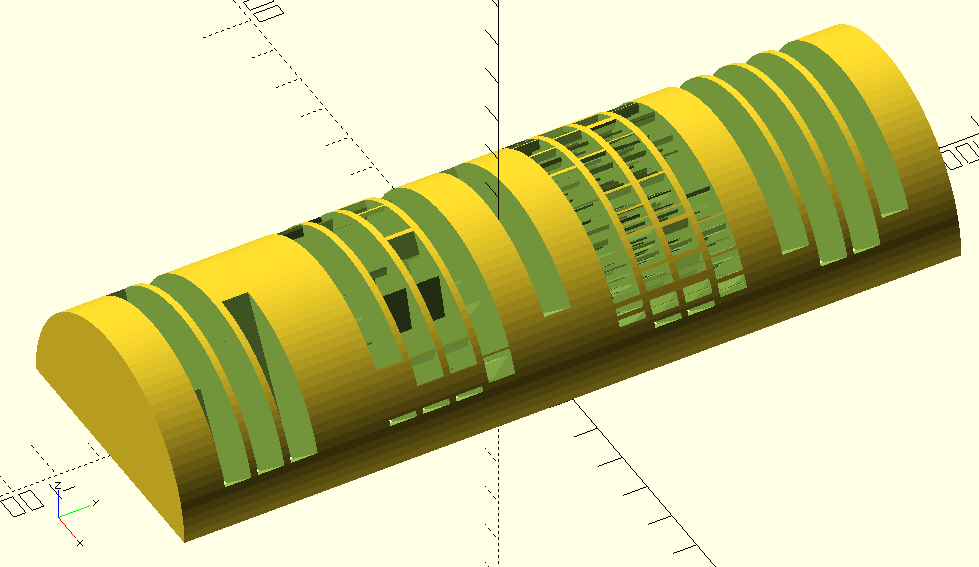
\includegraphics[width=.83\textwidth]{imagenes/reloj-de-sol-continuo-2}  
  \caption{La invocación del módulo \lstinline!reloj_de_sol! sin
    parámetros crea un reloj de Sol continuo...}
  \label{fig:reloj-de-sol-continuo-2}
\end{figure}


\begin{lstlisting}[numbers=none]
reloj_de_sol([[12,00],[7,13],[16,23]]);
\end{lstlisting}%


\begin{figure}[ht]
  \centering
  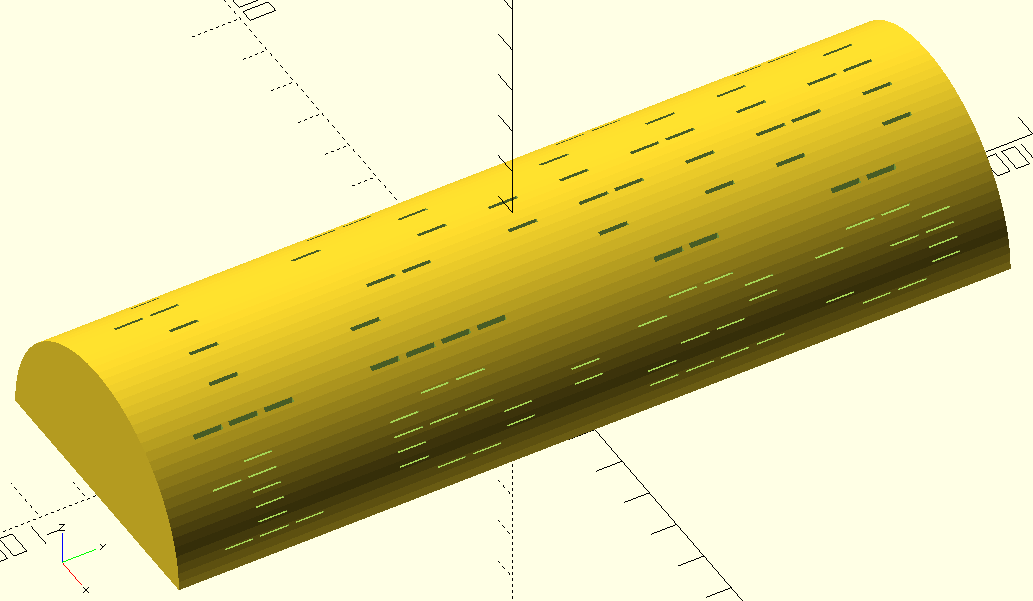
\includegraphics[width=.83\textwidth]{imagenes/reloj-de-sol-discreto-2}  
  \caption{...mientras que si se le ofrece un vector, produce un reloj de Sol discreto.}
  \label{fig:reloj-de-sol-discreto-2}
\end{figure}


---Está bueno ---aprobó Cecilia, mientras comenzaba a hacerse cargo de
su cuarta medialuna.

\section{Una vieja duda}

Antonia tomó la suya con la punta de sus dedos, para mancharlos lo
menos posible y así poder seguir escribiendo:

---No habrás olvidado tampoco una antigua duda que nos acompaña desde
el capítulo \ref{sec:el-primer-rayo-de-sol-ii}; se trataba del método
óptimo para ubicar correctamente el rayo de Sol, ahora mejor conocido
como `haz de Sol':

\begin{lstlisting}
module haz_de_sol(alfa1,alfa2){
  alfa_min=min(alfa1,alfa2);
  alfa_max=max(alfa1,alfa2);
  D1=H/tan(alfa_min);
  D2=H/tan(alfa_max);
  vertices=[[-alto_pixel/2,0],
            [D2-alto_pixel/2,H],
            [D1+alto_pixel/2,H],
            [alto_pixel/2,0]];
  // TODO: medir la duracion de esta solucion
  //       y la de esta otra:
  //       translate([0,ancho_pixel/2,0])
  //       Ojo : borrar 'center=true' abajo
  rotate ([90,0,0])
    linear_extrude(ancho_pixel,center=true)
      polygon(vertices);
}
\end{lstlisting}
  
Cecilia apenas se acordaba, pero se sintió obligada a asentir con
entusiasmo:

---Dale, compilemos ambas versiones y veamos.

Con la versión actual del texto el reloj completo demoraba un minuto y
medio en compilarse, mientras que la segunda versión tardaba...
virtualmente lo mismo:


\begin{figure}[ht]
  \centering
  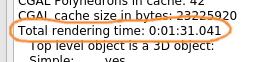
\includegraphics[width=.55\textwidth]{imagenes/tiempo-version-1}  
  \caption{Antonia comprueba el tiempo que demora la compilación del reloj...}
  \label{fig:tiempo-version-1}
\end{figure}




\begin{figure}[ht]
  \centering
  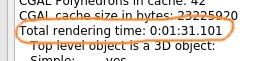
\includegraphics[width=.55\textwidth]{imagenes/tiempo-version-2}  
  \caption{...empleando las dos soluciones propuestas en el módulo
    \lstinline!haz_de_sol!.}
  \label{fig:tiempo-version-2}
\end{figure}


---La diferencia es ridícula; yo diría que elijamos la que nos guste
más ---propuso Antonia con despreocupación, dejando evidentemente la
decisión en manos de su amiga.

---Me gusta más la primera ---afirmó Cecilia, dando fin a su cuarta
medialuna.

\section{Texto}

---Si no me equivoco, me falta cumplir una última promesa: la
escritura de texto en \openscad{} ---dijo Antonia, mientras se
apresuraba a rescatar su quinta medialuna.

\begin{center}
\begin{minipage}[]{.55\textwidth}%\vspace{0pt}
 \begin{lstlisting}
linear_extrude(5)
  text("Cecilia Payne");
\end{lstlisting}%
\end{minipage}\hfill
%\begin{center}
\begin{minipage}[]{.45\textwidth}%\vspace{0pt}
  \centering
  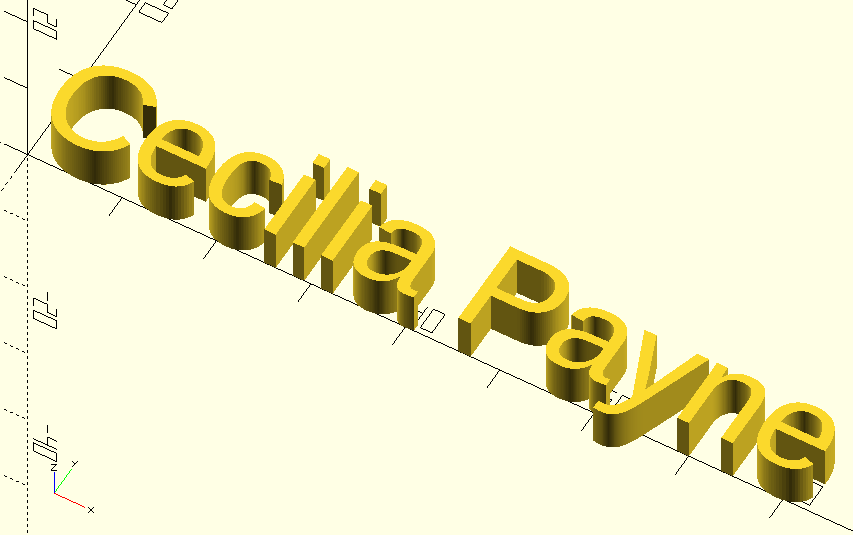
\includegraphics[width=1\textwidth]{imagenes/cecilia-payne}
\end{minipage}
\end{center}

\guillemotright La forma básica no puede ser más directa y sencilla:
consiste en usar la sentencia \lstinline!text! con el texto deseado
como parámetro ---señaló Antonia---. Esta sentencia, de por sí, crea
un objeto bidimensional, como lo hacen \lstinline!square!,
\lstinline!circle! y \lstinline!polygon!; por eso es necesario
otorgarle tridimensionalidad mediante una transformación como
\lstinline!linear_extrude!.

Tras una pausa para masticar, Antonia continuó:

---\lstinline!text! admite varios parámetros más.  Te sugiero
consultar el ayudamemoria de
\openscad{}\footnote{\url{https://openscad.org/cheatsheet/}} para
verlos todos; mientras tanto, te comento algunos.

\subsection{\texttt{size}}

\guillemotright Con \lstinline!size! podés indicar el tamaño de las
letras:

\begin{center}
\begin{minipage}[]{.55\textwidth}%\vspace{0pt}
 \begin{lstlisting}
for(s=[10:10:100])
  translate([0,10*s,0])
    linear_extrude(50)
      text("Cecilia Payne",size=s);
\end{lstlisting}%
\end{minipage}\hfill
%\begin{center}
\begin{minipage}[]{.45\textwidth}%\vspace{0pt}
  \centering
  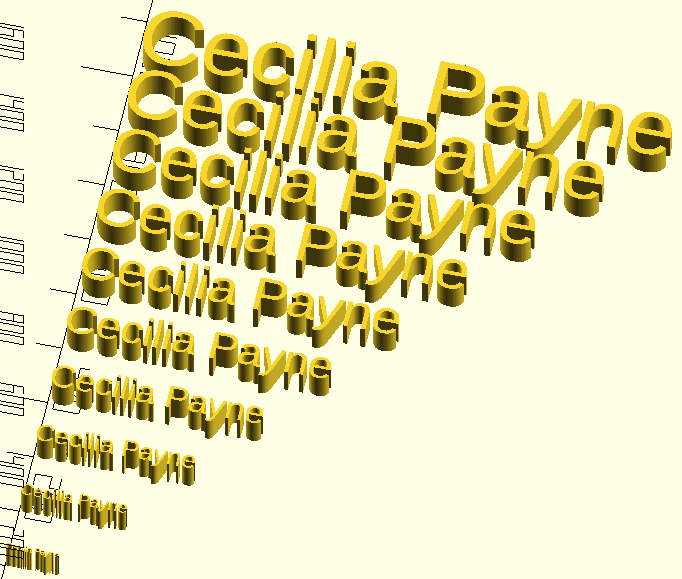
\includegraphics[width=1\textwidth]{imagenes/cecilia-payne-size}
\end{minipage}
\end{center}

\subsection{\texttt{valign}}

\guillemotright Con \lstinline!valign! es posible decidir la ubicación
de las letras respecto de la línea base; el valor por defecto es
\lstinline!baseline!.

\begin{center}
\begin{minipage}[]{.65\textwidth}%\vspace{0pt}
 \begin{lstlisting}[numbers=none]
text("Payne",valign="baseline");
\end{lstlisting}%
\end{minipage}\hfill
%\begin{center}
\begin{minipage}[]{.35\textwidth}%\vspace{0pt}
  \centering
  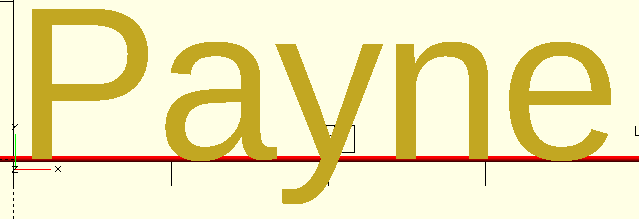
\includegraphics[width=.7\textwidth]{imagenes/payne-baseline}
\end{minipage}
\end{center}

\begin{center}
\begin{minipage}[]{.65\textwidth}%\vspace{0pt}
 \begin{lstlisting}[numbers=none]
text("Payne",valign="bottom");
\end{lstlisting}%
\end{minipage}\hfill
%\begin{center}
\begin{minipage}[]{.35\textwidth}%\vspace{0pt}
  \centering
  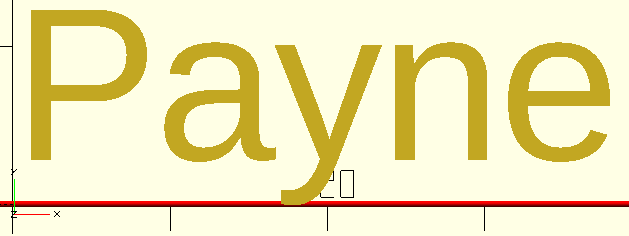
\includegraphics[width=.7\textwidth]{imagenes/payne-bottom}
\end{minipage}
\end{center}

\begin{center}
\begin{minipage}[]{.65\textwidth}%\vspace{0pt}
 \begin{lstlisting}[numbers=none]
text("Payne",valign="top");
\end{lstlisting}%
\end{minipage}\hfill
%\begin{center}
\begin{minipage}[]{.35\textwidth}%\vspace{0pt}
  \centering
  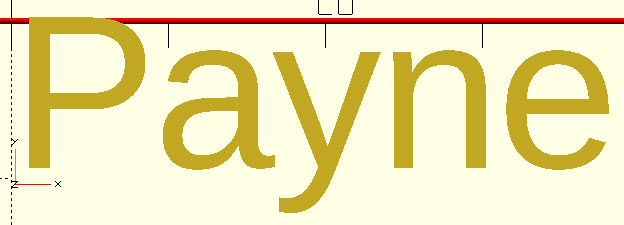
\includegraphics[width=.7\textwidth]{imagenes/payne-top}
\end{minipage}
\end{center}

\begin{center}
\begin{minipage}[]{.65\textwidth}%\vspace{0pt}
 \begin{lstlisting}[numbers=none]
text("Payne",valign="center");
\end{lstlisting}%
\end{minipage}\hfill
%\begin{center}
\begin{minipage}[]{.35\textwidth}%\vspace{0pt}
  \centering
  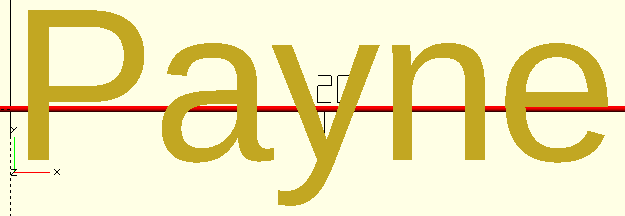
\includegraphics[width=.7\textwidth]{imagenes/payne-center-v}
\end{minipage}
\end{center}


\subsection{\texttt{halign}}

\guillemotright También es posible precisar la posición respecto de la
vertical; el valor por defecto es \lstinline!left!.


\begin{center}
\begin{minipage}[]{.65\textwidth}%\vspace{0pt}
 \begin{lstlisting}[numbers=none]
text("Payne",halign="left");
\end{lstlisting}%
\end{minipage}\hfill
%\begin{center}
\begin{minipage}[]{.35\textwidth}%\vspace{0pt}
  \centering
  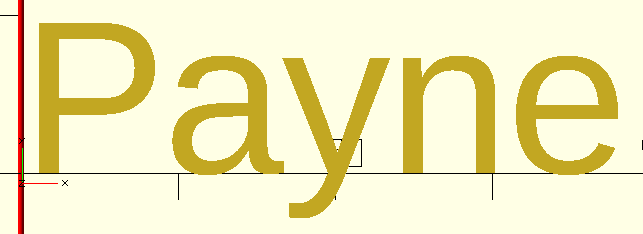
\includegraphics[width=.7\textwidth]{imagenes/payne-left}
\end{minipage}
\end{center}

\begin{center}
\begin{minipage}[]{.65\textwidth}%\vspace{0pt}
 \begin{lstlisting}[numbers=none]
text("Payne",halign="center");
\end{lstlisting}%
\end{minipage}\hfill
%\begin{center}
\begin{minipage}[]{.35\textwidth}%\vspace{0pt}
  \centering
  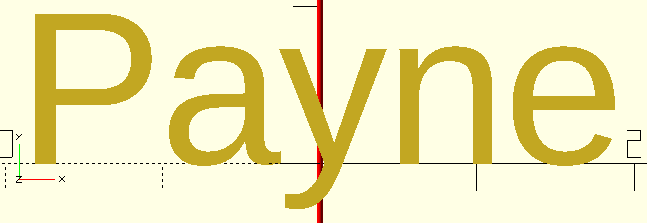
\includegraphics[width=.7\textwidth]{imagenes/payne-center-h}
\end{minipage}
\end{center}

\begin{center}
\begin{minipage}[]{.65\textwidth}%\vspace{0pt}
 \begin{lstlisting}[numbers=none]
text("Payne",halign="right");
\end{lstlisting}%
\end{minipage}\hfill
%\begin{center}
\begin{minipage}[]{.35\textwidth}%\vspace{0pt}
  \centering
  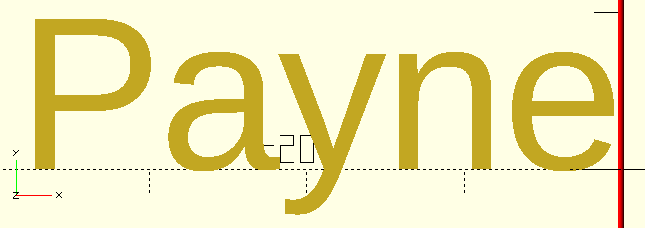
\includegraphics[width=.7\textwidth]{imagenes/payne-right}
\end{minipage}
\end{center}



\subsection{\texttt{font}}

\guillemotright Y, por supuesto, también podés elegir el tipo de
letra: tanto su familia como su estilo. Para eso primero tenés que ir
al menú \texttt{Ayuda} $\longrightarrow$ \texttt{Font List}, como podés
apreciar en la figura \ref{fig:menu-font-list}.


\begin{figure}[ht]
  \centering
  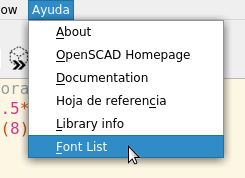
\includegraphics[width=.45\textwidth]{imagenes/menu-font-list}  
  \caption{Menú \texttt{Ayuda} $\rightarrow$ \texttt{font List}.}
  \label{fig:menu-font-list}
\end{figure}


\guillemotright Te aparecerá una larga lista de las fuentes presentes
en la computadora, igual o parecida a la de la figura
\ref{fig:font-list}; tenés que elegir una y hacer \emph{click} en el
botón `\texttt{Copiar al portapapeles}'.

\begin{figure}[ht]
  \centering
  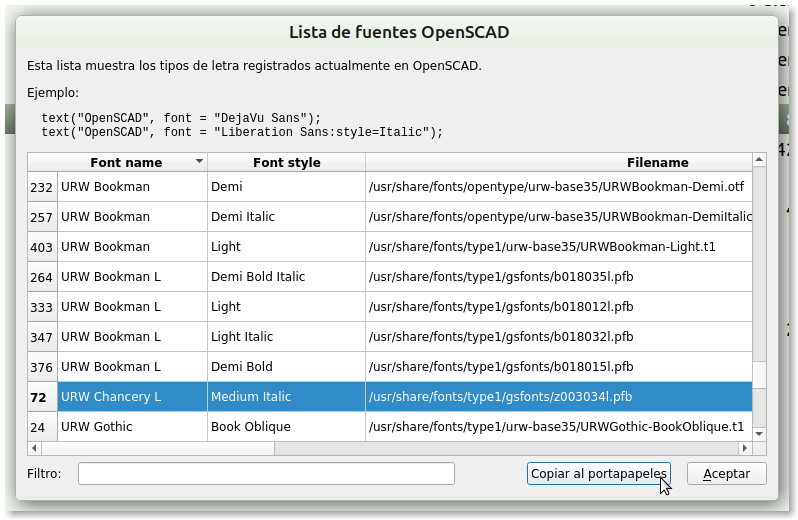
\includegraphics[width=.9\textwidth]{imagenes/font-list}  
  \caption{Lista de fuentes instaladas.}
  \label{fig:font-list}
\end{figure}


\guillemotright Ahora ya podés pegar el contenido del portapapeles,
entre comillas, luego del parámetro \lstinline!font!.

\begin{center}
\begin{minipage}[]{.49\textwidth}%\vspace{0pt}
 \begin{lstlisting}
linear_extrude(6)
  text("Cecilia Payne", font="URW Chancery L:style=Medium Italic");
\end{lstlisting}%
\end{minipage}\hfill
%\begin{center}
\begin{minipage}[]{.51\textwidth}%\vspace{0pt}
  \centering
  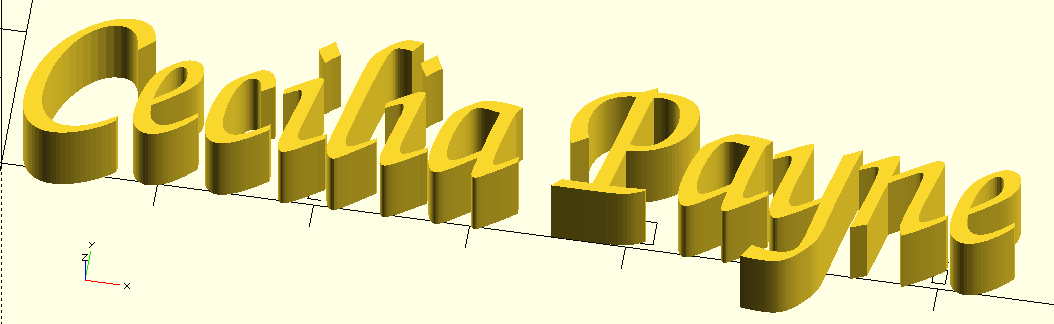
\includegraphics[width=1\textwidth]{imagenes/payne-font}
\end{minipage}
\end{center}

Cecilia saludó tan bello resultado dando los últimos mordiscos a su
quinta medialuna.

\section{La leyenda del reloj}

---Parece que la humanidad no considera una obra debidamente acabada
si no estampa sobre ella algunas palabras: placas conmemorativas en
edificios, frases motivadoras en jabones de tocador, patrocinios
publicitarios en camisetas deportivas son apenas unos ejemplos. Hasta
la música --que, como Borges le hizo decir a Schopenhauer, es la
única de las Artes que puede prescindir del Universo-- debe
sobrellevar las palabras: aunque Debussy impuso que los títulos de sus
preludios se imprimieran al pie de los mismos, no logró que dejáramos
de recordarlos por ellos ---Antonia suspiró, olvidando por un momento
que quedaban sólo dos medialunas.

\guillemotright Los relojes de Sol no son la excepción. Estuve
buscando una frase que diera algo de complejidad a sus bordes, pero
ninguna satisfizo mi vanidad: opté por escribir una propia.

Cecilia sintió que debía felicitar a su amiga:

---¿En serio?  ¡Qué bueno! ¿Y cuál fue?

Antonia sonrió, debidamente halagada:

---Por supuesto, debía ser en latín: \emph{Ab Revolutionibus Astri
  Girum Orbis Noscimus}.

Cecilia puso a prueba sus recuerdos colegiales de latín:

---¿Puede ser que signifique algo así como `De las revoluciones del
astro sabemos el giro del orbe'?

---A mí me gusta más `Gracias al giro (aparente) del Sol conocemos que
la Tierra rota' ---corrigió Antonia, sin disimular una nota de orgullo
en su voz.

---Me gusta ---concedió Cecilia, mientras miraba de reojo las dos
últimas medialunas.

Antonia buscó una imagen en su computadora; finalmente la encontró:

---Quería que quedara como en la figura \ref{fig:leyenda-1}.


\begin{figure}[ht]
  \centering
  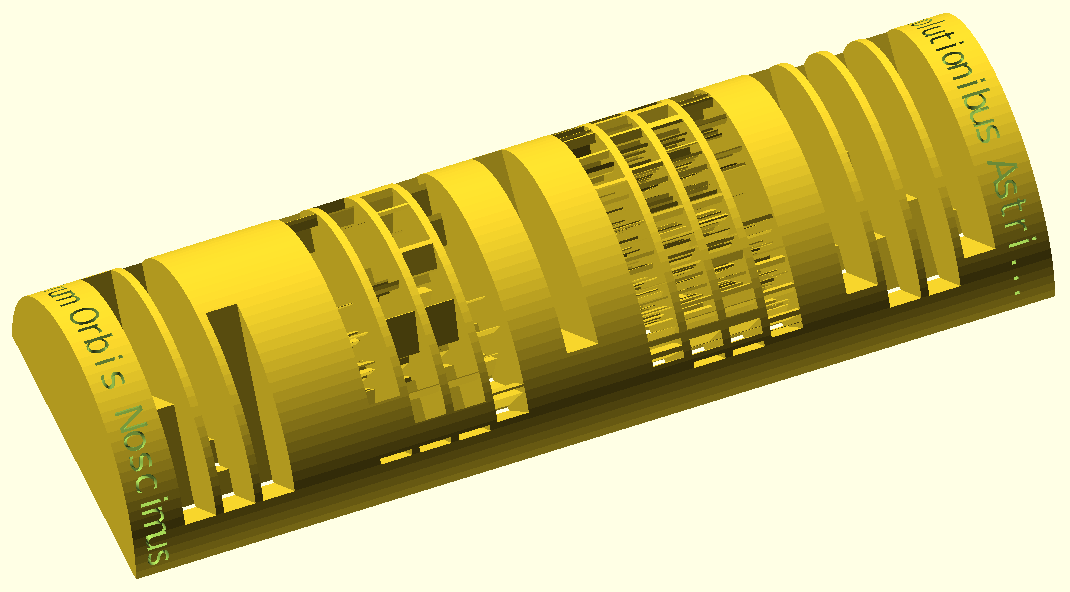
\includegraphics[width=1\textwidth]{imagenes/leyenda-1}  
  \caption{Antonia muestra cómo debería quedar la inscripción en los
    bordes del reloj.}
  \label{fig:leyenda-1}
\end{figure}


\guillemotright Tenemos entonces que escribir un módulo que despliegue
un texto a lo largo de un bonito arco circular ---agregó, mientras
cedía el teclado a Cecilia.

Ésta lo tomó y, olvidando también las últimas medialunas, comenzó a
pensar un voz alta:

---Yo diría que el módulo debería recibir el texto y su
tamaño... también su espesor, claro. ¡Ah! Y el radio del arco
circular, además del ángulo a lo largo del cual debe extenderse.

\begin{lstlisting}
module texto_circular(texto, size, espesor, radio, angulo){

}
\end{lstlisting}

\section{\texttt{len}}


<<Cada letra debería rotarse un cierto ángulo a lo largo del arco,
igual al ángulo total dividido por la cantidad de letras que tiene el
texto>> ---pensó Cecilia. En seguida agregó en voz alta, casi segura
de la respuesta:

---¿Hay una manera de calcular la longitud de un texto, Antonia?

Su amiga sonrió mientras recuperaba el teclado:

---Por supuesto; con la función \lstinline!len!:

\begin{center}
\begin{minipage}[]{.44\textwidth}%\vspace{0pt}
 \begin{lstlisting}[numbers=none]
echo(len("Hola"));
\end{lstlisting}%
\end{minipage}\hfill
%\begin{center}
\begin{minipage}[]{.55\textwidth}%\vspace{0pt}
  \centering
  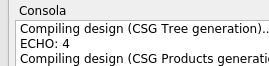
\includegraphics[width=1\textwidth]{imagenes/echo-len}
\end{minipage}
\end{center}

¡Perfecto! ---exclamó Cecilia, tomando el teclado.

\begin{lstlisting}
module texto_circular(texto, size, espesor, radio, angulo){
  longitud=len(texto);
  delta_alfa=angulo/longitud;
}
\end{lstlisting}

Antonia no esperó esta vez a que Cecilia la mirara para expresar su
disconformidad:

---Hmm... no estoy de acuerdo. Los `huecos' entre letras son uno menos
que la cantidad de éstas; por ejemplo, si tu texto tuviera dos letras,
\lstinline!delta_alfa! debería ser igual a \lstinline!angulo!, no a su
mitad.

Cecilia admitió con una sonrisa que su amiga tenía razón.

\begin{lstlisting}
module texto_circular(texto, size, espesor, radio, angulo){
  longitud=len(texto);
  delta_alfa=angulo/(longitud-1);
}
\end{lstlisting}

<<Ahora tengo que recorrer las letras del texto, una por una, para
crearlas, desplazarlas y rotarlas>> ---pensó. Y segura de que eso
tenía que ser posible, preguntó:

---¿Cómo hago para rescatar del texto una letra en particular?

---Las cadenas de texto son tratadas por \openscad{} como vectores de
caracteres, por lo que podés obtener uno cualquiera empleando un
índice ---explicó Antonia, mientras volvía a tomar el teclado.

\begin{center}
\begin{minipage}[]{.7\textwidth}%\vspace{0pt}
 \begin{lstlisting}
texto="abcdefgh";
echo(texto[0],texto[4],texto[2]);
\end{lstlisting}%
\end{minipage}\hfill
%\begin{center}
\begin{minipage}[]{.3\textwidth}%\vspace{0pt}
  \centering
  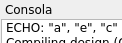
\includegraphics[width=.85\textwidth]{imagenes/echo-texto-i}
\end{minipage}
\end{center}


---¡Genial! ---aprobó Cecilia recobrando el teclado una vez más.

\begin{lstlisting}
module texto_circular(texto, size, espesor, radio, angulo){
  longitud=len(texto);
  delta_alfa=angulo/(longitud-1);
  for(i=[0:longitud-1]){
 
  }
}
\end{lstlisting}

---Ya es la segunda vez que aparece \lstinline!longitud-1!...
---pro\-tes\-tó Antonia---. ¿Y si en lugar de almacenar la longitud del
texto guardás ese otro valor aparentemente más útil?

Cecilia no encontró reparos en aceptar la sugerencia.

\begin{lstlisting}
module texto_circular(texto, size, espesor, radio, angulo){
  n=len(texto)-1;
  delta_alfa=angulo/n;
  for(i=[0:n]){

  }
}
\end{lstlisting}

---De paso, tipeo menos ---bromeó---. Ahora sí: a cada letra la separo
del origen una distancia igual a \lstinline!radio!, y la roto
\lstinline!delta_alfa*i! grados.

\begin{lstlisting}
module texto_circular(texto, size, espesor, radio, angulo){
  n=len(texto)-1;
  delta_alfa=angulo/n;
  for(i=[0:n])
    rotate([0,0,delta_alfa*i])
      translate([radio,0,0])
        linear_extrude(espesor)
          text(texto[i], size=size, font="DejaVu Sans:style=Book");
}

\end{lstlisting}

Cada letra era creada en las líneas 7 y 8, alejada del centro en la 6
y rotada en la 5.

\begin{lstlisting}[numbers=none]
texto_circular(texto="Ab Revolutionibus Astri...", size=5, espesor=3, radio=60, angulo=90);
\end{lstlisting}


\begin{figure}[ht]
  \centering
  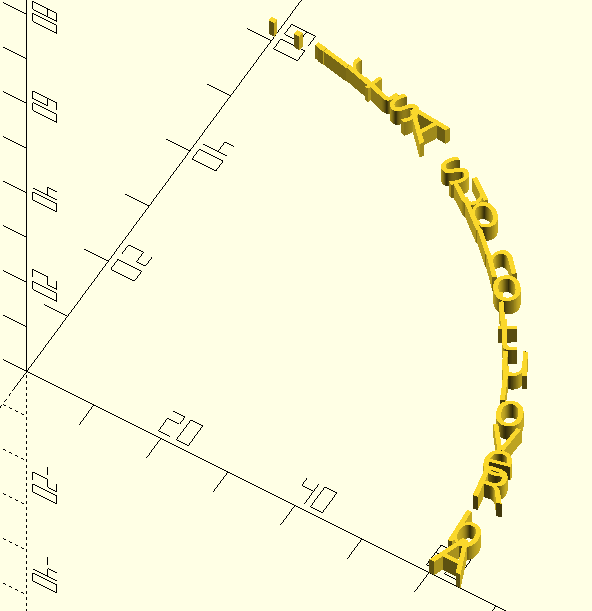
\includegraphics[width=.7\textwidth]{imagenes/texto-circular-1}  
  \caption{El texto es efecticamente circular, pero las letras no
    están dispuestas como esperamos.}
  \label{fig:texto-circular-1}
\end{figure}


El resultado, tal como podía apreciarse en la figura
\ref{fig:texto-circular-1}, era efectivamente un texto dispuesto
circularmente, pero no como ella lo esperaba: las letras debían
presentar su dorso al centro, y estar alineadas con el eje de
rotación.

---Supongo que tengo que rotar las letras antes de trasladarlas
---aventuró, y se dispuso a intercalar una línea más.

\begin{lstlisting}
module texto_circular(texto, size, espesor, radio, angulo){
  n=len(texto)-1;
  delta_alfa=angulo/n;
  for(i=[0:n])
    rotate([0,0,delta_alfa*i])
      translate([radio,0,0])
        rotate([90,0,90])
          linear_extrude(espesor)
            text(texto[i], size=size, font="DejaVu Sans:style=Book");
}
\end{lstlisting}


\begin{figure}[ht]
  \centering
  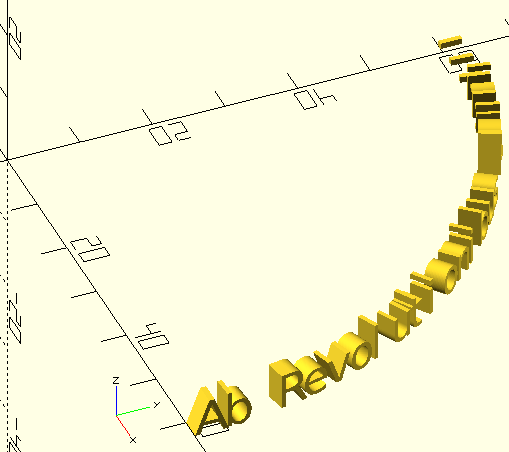
\includegraphics[width=.7\textwidth]{imagenes/texto-circular-2}  
  \caption{Ahora las letras presentan correctamente su dorso al eje de
    rotación.}
  \label{fig:texto-circular-2}
\end{figure}


---¡Mucho mejor! ---exclamó Cecilia admirando complacida la figura
\ref{fig:texto-circular-2}, mientras tomaba triunfalmente su sexta
medialuna y la apoyaba frente a su boca como una sonrisa subrayada,
antes de darle un implacable mordisco.

Antonia aplaudió con entusiasmo antes de oponer un par de objeciones y
hacerse cargo de la medialuna restante:

---Fijate que el arco comienza justo en el eje \coord{X} y, pese a que
indicaste un ángulo de 90$^{\circ}$, el último punto se pasó un
poquito del eje \coord{Y}.

Cecilia pudo verlo, pero no así el inconveniente.

---Esto pasa porque cada letra, por defecto, está alineada
horizontalmente `por izquierda'; yo diría que resulta más natural que
cada letra esté centrada ---argumentó Antonia.

Cecilia ahora entendió la observación, y no le costó nada salvarla.

\begin{lstlisting}
module texto_circular(texto, size, espesor, radio, angulo){
  n=len(texto)-1;
  delta_alfa=angulo/n;
  for(i=[0:n])
    rotate([0,0,delta_alfa*i])
      translate([radio,0,0])
        rotate([90,0,90])
          linear_extrude(espesor)
            text(texto[i], size=size, font="DejaVu Sans:style=Book", halign="center");
}
\end{lstlisting}


\begin{figure}[ht]
  \centering
  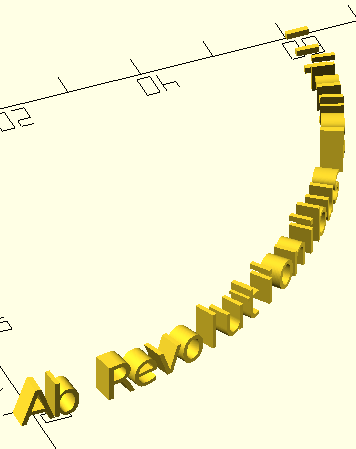
\includegraphics[height=.54\textwidth]{imagenes/texto-circular-3}\hfill
  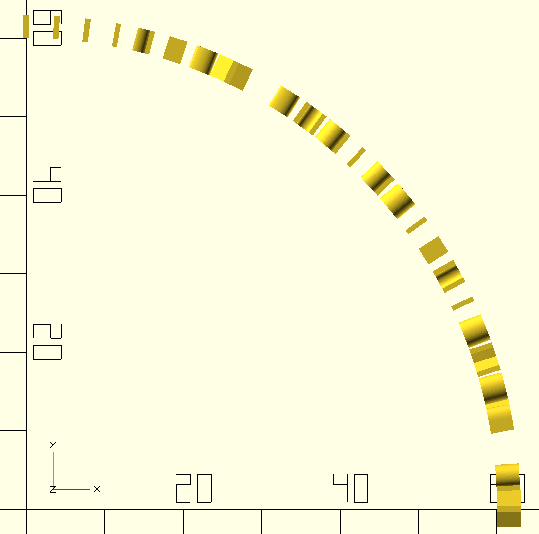
\includegraphics[height=.54\textwidth]{imagenes/texto-circular-4}  
  \caption{Las letras ahora están alineadas horizontalmente de manera
    correcta.}
  \label{fig:texto-circular-3-4}
\end{figure}


---Fue tan fácil como agregar un \lstinline!halign=``center''! en la
línea 9 ---comentó complacida, enseñando a su amiga la figura
\ref{fig:texto-circular-3-4}.

---Una última cuestión ---prometió Antonia, señalando a su vez la
figura \ref{fig:texto-plano-yz}---.  Nosotras queremos que el texto
quede centrado respecto del eje longitudinal del reloj; es decir,
queremos que resulte simétrico respecto del plano \coord{YZ}.  Yo
diría que para lograr eso conviene que el módulo
\texttt{texto\_cir\-cular} produzca un texto simétrico respecto del
plano \coord{XZ}; en otras palabras, que no empiece en el eje
\coord{X}, sino un ángulo igual a \lstinline!angulo/2! antes
---explicó Antonia.



\begin{figure}[ht]
  \centering
  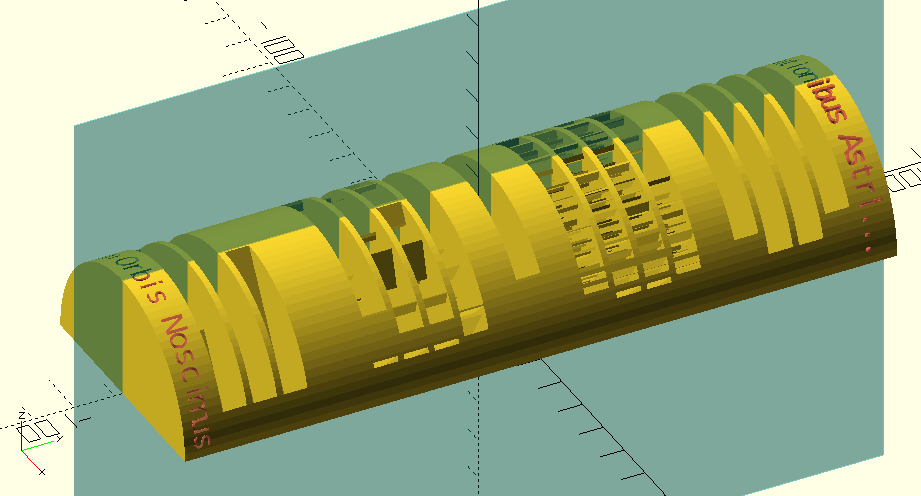
\includegraphics[width=.9\textwidth]{imagenes/texto-plano-yz}  
  \caption{El texto deberia resultar simétrico respecto del plano
    \coord{YZ}}
  \label{fig:texto-plano-yz}
\end{figure}

A Cecilia le pareció razonable.

\begin{lstlisting}
module texto_circular(texto, size, espesor, radio, angulo){
  n=len(texto)-1;
  delta_alfa=angulo/n;
  for(i=[0:n])
    rotate([0,0,delta_alfa*i-angulo/2])    
      translate([radio,0,0])
        rotate([90,0,90])
          linear_extrude(espesor)
            text(texto[i], size=size, font="DejaVu Sans:style=Book", halign="center");
}
\end{lstlisting}

Sólo fue necesario modificar la línea 5: todas las letras recibían una
rotación extra de \lstinline!-angulo/2! grados.

\begin{lstlisting}[numbers=none]
texto_circular(texto="Ab Revolutionibus Astri...", size=5, espesor=3, radio=60, angulo=90);
\end{lstlisting}


\begin{figure}[ht]
  \centering
  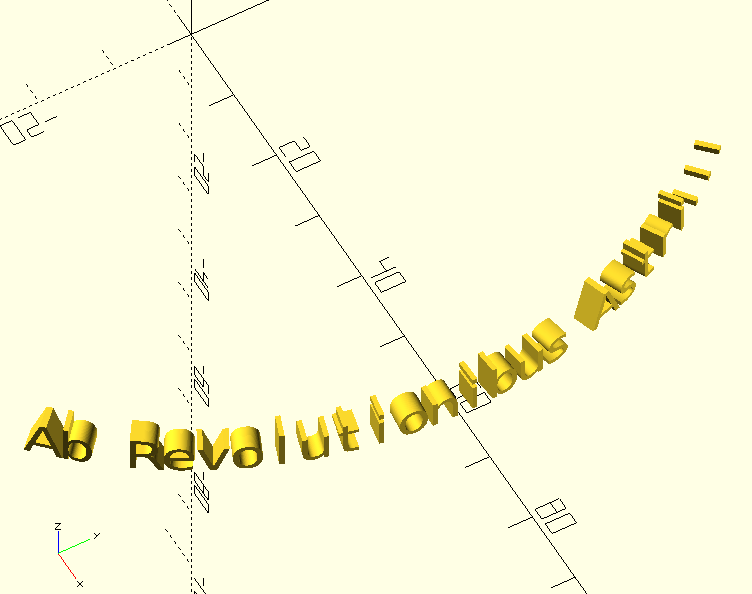
\includegraphics[width=.6\textwidth]{imagenes/texto-circular-6}  
  \caption{El texto producido por el módulo \lstinline!texto_circular!
    resulta ahora simétrico al plano \coord{XZ}.}
  \label{fig:texto-circular-6}
\end{figure}


% \begin{lstlisting}
% texto_circular(texto="Ab Revolutionibus Astri...", size=5, espesor=3, radio=60, angulo=180);
% \end{lstlisting}

% \begin{center}
%   \includegraphics[width=.4\textwidth]{imagenes/texto-circular-180}
% \end{center}

---¡Excelente! ---esta vez Antonia, contemplando la figura
\ref{fig:texto-circular-6}, no tuvo nada que ob\-je\-tar.

---Creo que el texto debería poder ser elegido por el usuario ---opinó
Cecilia---. Vamos a guardarlo en dos variables, junto con las demás.

\begin{lstlisting}
texto_1 = "Ab Revolutionibus Astri...";
texto_2 = "...Girum Orbis Noscimus";
\end{lstlisting}

Cecilia no estaba tan segura de que en latín todas las palabras
llevaran mayúscula inicial, pero no se sentía tan solvente en
gramática clásica como para contradecir a su amiga.% \footnote{El lector
  % perspicaz tal vez logre descifrar en esas iniciales una suerte de
  % mensaje más o menos secreto. (Nota del Autor)}$^,$\footnote{¿En
  % serio? ¡Me encantan los mensajes secretos! ¿De qué se trata? (nota
  % del Editor)}$^,$\footnote{Hmmm... ¿Sabés guardar un
  % secreto?}$^,$\footnote{¡Claro!}$^,$\footnote{Yo
  % también.}$^,$\footnote{¡Ufa!}

\section{\texttt{import}}

---Ahora debemos aplicar ambos textos circulares al cuerpo del
reloj. El problema es que para ver cómo va quedando deberíamos
compilar el reloj a cada paso ---Antonia no parecía querer someter a
su computadora a los mismos cálculos una y otra vez---. Así que estaría
bueno poder guardar el reloj como un objeto compilado aparte, y usarlo
luego como si fuera un cuerpo básico más ---y tomó el teclado para
sí, dispuesta a volver ese deseo realidad.

\guillemotright Una vez que creamos el reloj con \keystroke{F6}
podemos grabarlo en la computadora con \keystroke{F7} o usando el
icono correspondiente de la barra ---mostró Antonia, señalando la
figura \ref{fig:exportar-stl}.


\begin{figure}[ht]
  \centering
  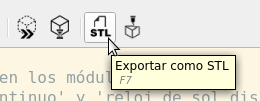
\includegraphics[width=.55\textwidth]{imagenes/exportar-stl}  
  \caption{Icono para exportar un objeto en formato \textsc{STL}.}
  \label{fig:exportar-stl}
\end{figure}


\guillemotright De paso te cuento que el formato \texttt{.STL} es nada
menos que el que debemos producir en última instancia para procesarlo
luego mediante un programa que lo traduzca al lenguaje que las
impresoras 3D entienden ---explicó---. Pero ahora nos interesa porque
este tipo de archivos podemos incluirlo en nuestras escenas usando la
sentencia \lstinline!import!.

\begin{figure}[ht]
\begin{minipage}[]{.5\textwidth}%\vspace{0pt}
 \begin{lstlisting}[numbers=none]
import("reloj-de-sol.stl");
\end{lstlisting}%
\end{minipage}\hfill
%\begin{center}
\begin{minipage}[]{.46\textwidth}%\vspace{0pt}
  \centering
  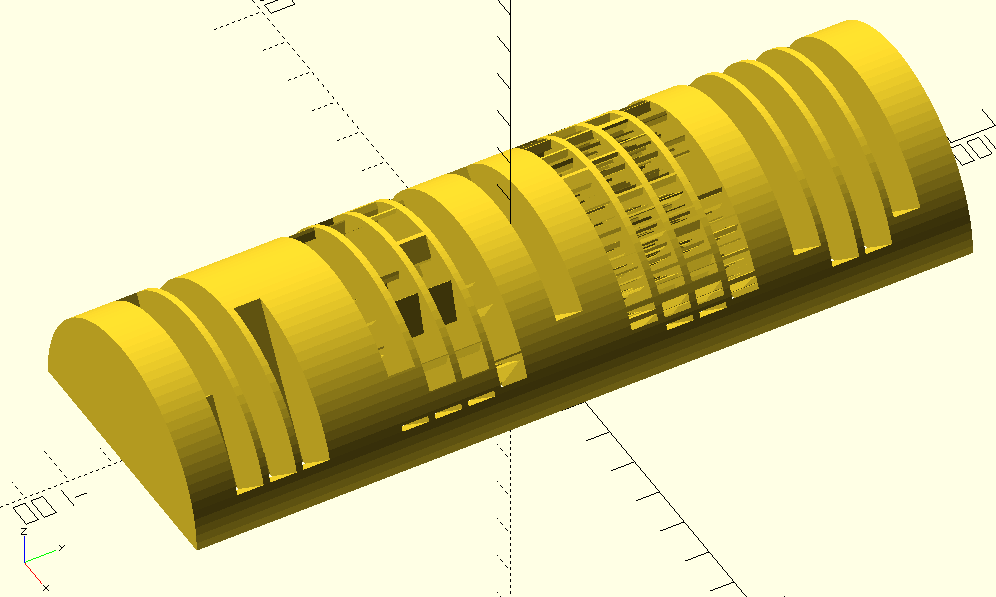
\includegraphics[width=\iftoggle{libro}{.75}{1}\textwidth]{imagenes/reloj-de-sol-import}
\end{minipage}
\caption{Antonia demuestra cómo importar un archivo en formato
  \textsc{STL} dentro de una escena.}
  \label{fig:reloj-de-sol-import}
\end{figure}


\guillemotright En el ejemplo de la figura
\ref{fig:reloj-de-sol-import}, `\texttt{reloj-de-sol.stl}' es el
nombre que le dimos al archivo cuando lo grabamos con \keystroke{F7}
---a\-cla\-ró Antonia.

---Sí, me doy cuenta ---Cecilia pudo verlo de inmediato, y recobró el
teclado dispuesta a estampar sobre los bordes del reloj la frase de
Antonia. Se valió del modificador `\lstinline!#!' para poder ver los
textos a medida que los movía; después de unos minutos de tanteos,
logró un resultado que la satisfizo.

\begin{lstlisting}
difference(){
  import("reloj-de-sol.stl", convexity=3);
  #translate([0,largo_reloj/2-borde+2.5,0])
    rotate([0,-90,-90])
      texto_circular(texto_1,5,2, radio_semicilindro-1.2,165);
  #translate([0,-largo_reloj/2+2.5,0])
    rotate([0,-90,-90])
      texto_circular(texto_2,5,2, radio_semicilindro-1.9,165); 
}
\end{lstlisting}


\begin{figure}[ht]
  \centering
  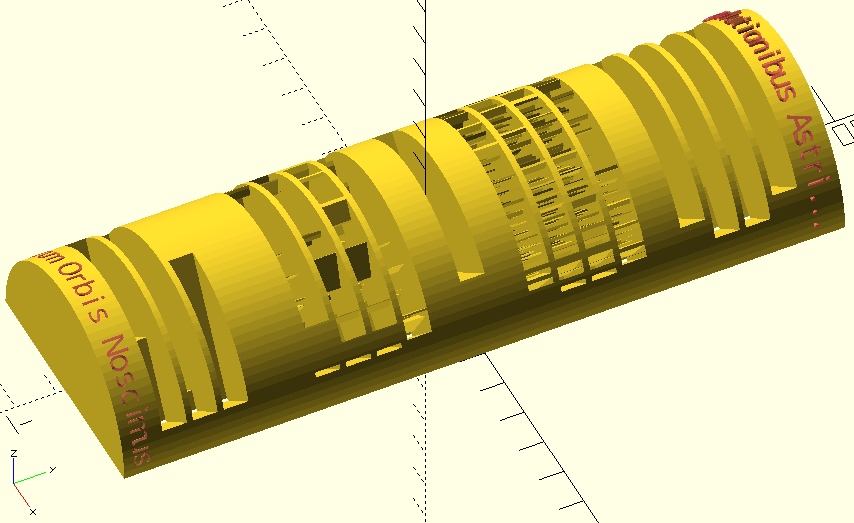
\includegraphics[width=.9\textwidth]{imagenes/reloj-de-sol-con-leyendas-1}  
  \caption{Cecilia estampa en los bordes del reloj las leyendas de
    Antonia.}
  \label{fig:reloj-de-sol-con-leyendas-1}
\end{figure}


En la línea 2, por consejo de Antonia, incluyó el parámetro
\lstinline!convexity=3!: resultaba misteriosamente necesario para que
el reloj no se viera como en la figura \ref{fig:import-sin-convexity}.


\begin{figure}[ht]
  \centering
  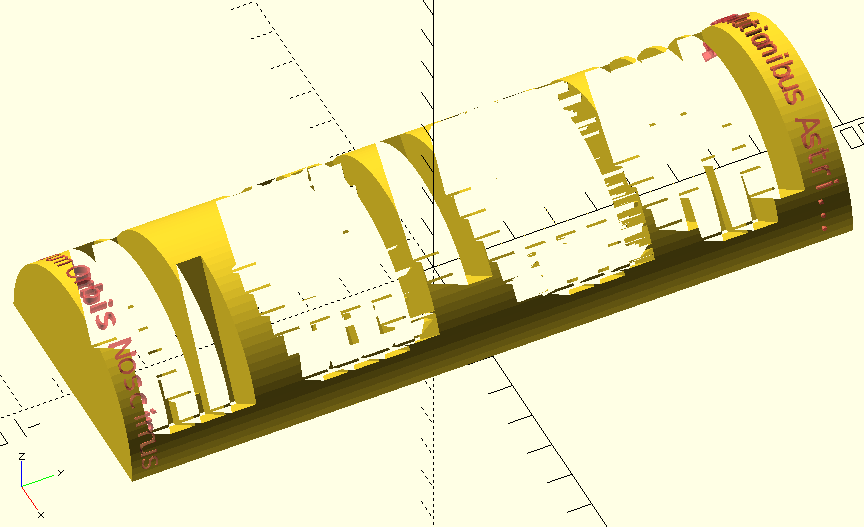
\includegraphics[width=.8\textwidth]{imagenes/import-sin-convexity} 
  \caption{Si se emplea la sentencia \lstinline!import! sin dar a la
    opción \texttt{convexity} un valor mayor a 1, los objetos
    importados pueden manifestarse de forma anómala.}
  \label{fig:import-sin-convexity}
\end{figure}


Las líneas 4 y 7 servían para rotar las leyendas a fin de que
discurrieran en torno al eje longitudinal del reloj; las líneas 3 y 6
las trasladaban a los bordes del mismo. El radio de cada texto era
igual a \lstinline!radio_semicilindro-1.9! porque el espesor de cada
letra era igual a 2, y Cecilia quería que sobresalieran apenas del
cuerpo del reloj a fin de que la sentencia \lstinline!difference! no
se encontrara frente la dificultosa ambigüedad de las superficies
coincidentes.

---Perfecto ---aprobó Antonia---. Ahora que comprobamos que funciona,
debemos incluir ese código en el módulo \lstinline!reloj_de_sol!.

Cecilia estaba completamente de acuerdo.

\begin{lstlisting}
module reloj_de_sol(vector_horas){
  difference(){
    // Reloj
    if(vector_horas==undef)
      reloj_de_sol_continuo();
    else
      reloj_de_sol_discreto(vector_horas);
    // Textos
    translate([0,largo_reloj/2-borde+2.5,0])
      rotate([0,-90,-90])
        texto_circular(texto_1,5,2, radio_semicilindro-1.2,165);
    translate([0,-largo_reloj/2+2.5,0])
      rotate([0,-90,-90])
        texto_circular(texto_2,5,2, radio_semicilindro-1.9,165);
  }
}
reloj_de_sol();
\end{lstlisting}%


\begin{figure}[ht]
  \centering
  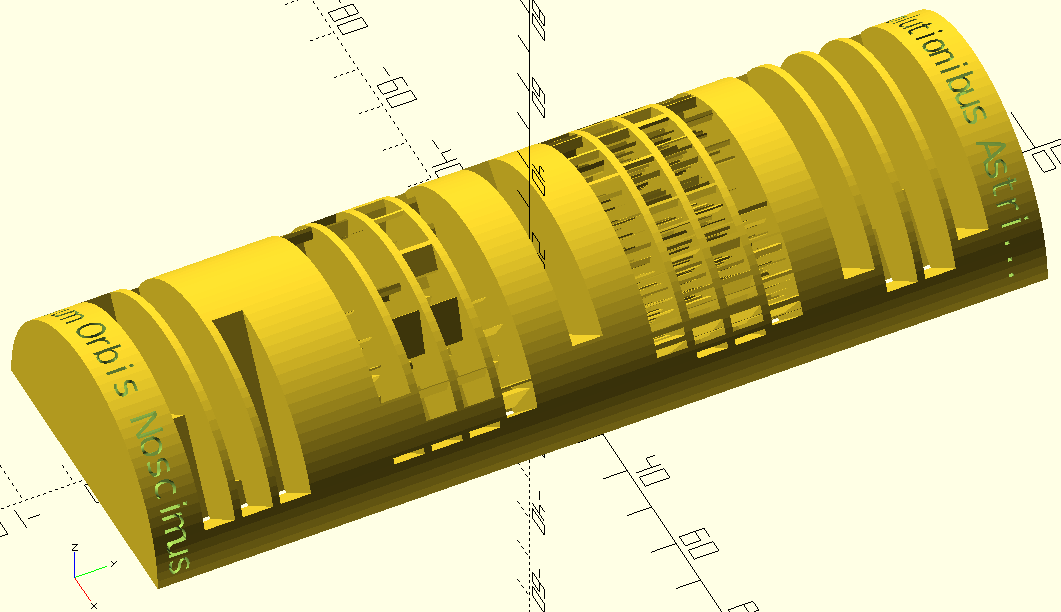
\includegraphics[width=1\textwidth]{imagenes/reloj-con-leyendas-2}  
  \caption{Reloj de Sol con las leyendas impresas en los bordes.}
  \label{fig:reloj-con-leyendas-2}
\end{figure}


\section{Firma}

Las últimas medialunas habían desaparecido ya a través del tracto
digestivo de ambas amigas, dejando tras sí como únicos testigos unas
cuantas miguitas indiscretas en el escritorio.

Cecilia miraba su reloj de Sol con una serena felicidad, que no supo
si atribuir a la dicha de haberlo concluido exitosamente o a la
espléndida digestión.

Antonia, por su parte, no parecía ahora compartir su felicidad; antes
bien, una sombra de melancolía ensombrecía su rostro. Casi con
desgano, propuso lentamente:

---Nuestra vanidad no sería colmada si renunciamos a firmar un objeto
tan soberbio como nuestro reloj ---y agregó unas últimas líneas al
texto que comenzaran a escribir tantos capítulos atrás, sin que ya las
teclas sonaran bajo sus dedos con la alegría pasada.


\begin{figure}[ht]
  \centering
  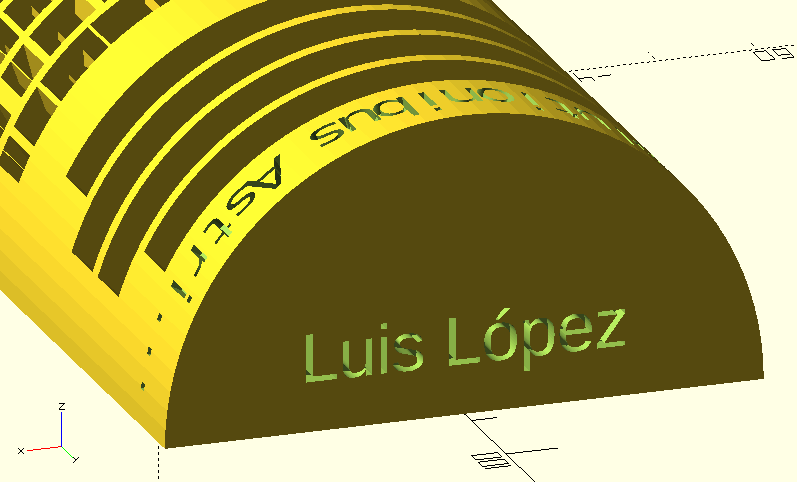
\includegraphics[width=.6\textwidth]{imagenes/firma}  
  \caption{La firma del autor.}
  \label{fig:firma}
\end{figure}


Cecilia arqueó las cejas con extrañeza ante la figura \ref{fig:firma}.

---¿Y eso?  ---preguntó.

Antonia tardó un instante en responder; su voz tenía un tinte opaco:

---La firma del autor.

Cecilia se irguió lentamente en su silla. Un incierto malestar comenzó
a recorrer su cuerpo; casi temió preguntar:

---¿A qué te referís, Antonia? No entiendo la broma ---y trató de
sonreír, pero notó que le costaba.

Su amiga giró hacia ella con lentitud antes de mirarla fijamente a los
ojos:

---Este reloj lo escribió Luis, tu profesor de Astronomía ---y ante la
muda mirada de Cecilia, prosiguió---: Este es un manual mediocre que
se propuso escribir para dejar constancia de su obra, nada
más. Nosotras no existimos.

Cecilia sintió que un sudor frío se apoderaba de su frente. Quiso
reír, pero nuevamente algo la contuvo. Fue como si todo su íntimo ser
conociera desde siempre el significado de lo que, a todas luces, no
debería haber sido otra cosa que una broma estúpida de Antonia

---No es gracioso ---fue todo lo que pudo balbucear, nerviosa.

---No estoy diciendo que lo sea: la realidad no tiene la obligación de
ser graciosa. Pero es real ---Antonia pareció agitarse; con un tono
ligeramente vibrante, añadió---: Y vos lo sabés, Cecilia: ¿Porqué
durante todo este tiempo hicimos referencia, tanto vos como yo, a
`capítulos'? ¿Cómo hice para `leerte la mente' tantas veces? ---se
desplomó contra el respaldo de su silla, y con voz nuevamente calma,
agregó---: Somos personajes, Cecilia. Simples personajes. Ni siquiera
bien construidos; somos casi de cartón. Nosotras... no
existimos\footnote{¿Yo tampoco..?  (Nota del Editor)}$^,$\footnote{Vos
  tampoco: ¿quién hallará editor para este manualcito?} ---y estas
últimas palabras escaparon de su boca como un suspiro.

La mente de Cecilia se vio arremetida por un huracán de incertidumbre
y rebeldía; quería indignarse con su amiga, agitarse contra ella. No
quería aceptarlo: no podía ser verdad. Con gran esfuerzo trató de
serenarse. <<Cecilia, sos una científica>> ---se dijo a sí
misma---. <<Apelá a tu capacidad de demostración>>.

Respirando hondo, argumentó:

---Mirá, Antonia ---procuró que su voz sonara calma; no lo
logró---. Acá estoy: mirame. Existo. E--xis--to.

Apenas pronunciadas estas palabras se sintió tonta al descubrirse
tratando de demostrar su existencia separando en sílabas un verbo. Con
inquietud recorrió la oficina con la mirada: sus ojos se detuvieron en
el vacío dejado por las medialunas.

---¡Acabamos de comer medialunas!  ---proclamó con tono
triun\-fal---. ¿Los fantasmas comen medialunas, acaso?

Antonia le devolvió la mirada con una sonrisa triste y dulce:

---¿De qué eran las medialunas? ---y su voz era apenas un susurro.

Cecilia sintió que una mano helada se cerraba sobre su corazón:

---¿Cómo de qué eran? ---preguntó con voz quebrada, aunque entendía
perfectamente el significado de la pregunta.

---Sí, de qué eran: ¿de grasa o de manteca? ---en la voz de Antonia
flotaba una delicada ternura.

Cecilia cubrió su rostro con las manos:

---Basta.... basta... ---suplicó.

Un silencio pesado envolvió a las amigas. El Sol comenzaba a ponerse,
y sus débiles rayos ingresaban por la alta...

---¡Basta, dije! ---gritó Cecilia---. ¡Esto no puede terminar así!
¡Manual o no manual, esto no puede terminar así!

El grito de Cecilia me molestó menos que su redundancia: ¿No podía
haber utilizado el verbo ``concluir'' en la tercera exclamación? Como
sea, decía que el Sol comenzaba...

---¡NO! ---Cecilia se puso de pie en medio de la oficina---.  ¡Dije
que no, Luis!

Esto no está concluyendo como esperaba, evidentemente. Antonia también
se levantó; espero que tranquilice a Cecilia y podamos cerrar el
capítulo y el manual como corresponde y en paz.

---No es tan malo como parece ---Antonia apeló a la empatía para
sosegar a su amiga---. Ya nos ocurrió con el manual del \annielogo{},
y aquí estamos. Y seguramente volveremos a estar en algún otro manual
tan malo como estos.

Cecilia se agitó con cierta violencia; esta vez parecía pasar algo
más:

---¡No! ¡Me niego! ---exclamó con firmeza; en su voz ya no había
nerviosismo---. Quizá no pueda demostrarlo. Quizá sea más natural
aceptar que somos un manojo de palabras. Pero yo sé que no es así: yo
existo ---pareció morder esta última palabra; tras girar bruscamente
hacia su amiga, añadió---: Y vos también, Antonia: vos existís.

Confieso que a esta altura ya estoy inquiétandome un poco; más que
nada porque estamos en la página
\pagedifferenceplusone{sec:texto}{sec:texto-b} del
capítulo\label{sec:texto-b} y quería ir cerrándolo. Pero debo admitir
también que se ha despertado en mí una cierta sensación de divertida
hilaridad. Esta situación incluso me recuerda algo...\footnote{¡La
  novela \emph{Niebla}, de Miguel de Unamuno! ¡Plagio! (nota del
  Editor)}$^,$\footnote{Novela, no: nivola. Pero es verdad: me
  recuerda ese libro. Y no seas resentido: no es plagio. Digamos que
  es un... ¿homenaje?}

Cecilia caminaba por la oficina; sus pasos sonaban con firmeza contra
el piso de madera. Sus ojos brillaban con el fuego de un pensamiento
intenso y voraz. Antonia, inmóvil, la seguía con una mirada dulce y
comprensiva.

Cecilia detuvo de golpe sus pasos:

---¡Ya sé! ---exclamó---. Luis sigue trabajando aquí, en Harvard, ¿no?
---y en su mirada una luz de feroz intensidad se abrió paso.

---Sí; en el Observatorio ---contestó Antonia---. ¿Por qué?
---pre\-gun\-tó a continuación y con cautela.

Cecilia no respondió inmediatamente. Respiró con fuerza, y
dirigiéndose con decisión hacia la puerta aseguró:

---Para hacerle una visita. ¿Venís?

Y antes de que pudiera terminar el capítulo, juntas abandonaron la
oficina y se dirigieron al Observatorio de Harvard, donde acabo de
enterarme de que las estoy esperando.



%%% Local Variables:
%%% mode: latex
%%% TeX-master: "../libro"
%%% End:
